\chapter{Design and Implementation}\label{C:workdone}

\section{Overview}

The ability to trace java unit tests and perform several different analysis metrics has been implemented. For this to be achieved, several factors had to be completed and these are explored in this chapter. The different types of spectra are looked at in Section \ref{S:spectra}. The different types of analysis metrics are explored in Section \ref{S:metrics}. How the tracing is performed is examined in Section \ref{S:trace}, while the creation of the framework is explored in Section \ref{S:framework}. Lastly, how the benchmarks were selected is looked at in Section \ref{S:bench}.

\section{Test Spectra}
\label{S:spectra}

The idea of a spectrum was previously identified in Chapter \ref{C:intro}. A spectrum is some abstraction of the method executions during a test. This allows there to be several different types of spectra. The main three spectra examined are set, list and calling context. An example using the word kitten will be used to show them, where each letter represents a method execution and each letter is from the same parent method.

\begin{itemize}
\item Set of method executions - where every method execution is only taken into account once (Result: 'Kiten')
\item List of method executions - where every method execution is taken into account, including duplicate calls (Result : 'Kitten')
\item Calling Context - for each method call, the data contains a separate node for each call stack that the method was called with \cite{callingcontext} (Result : 'Parent $\rightarrow$ k, Parent $\rightarrow$ i, Parent $\rightarrow$ t ...) 
\end{itemize}
These spectra will be analysed by different metrics to determine the level of redundancy between two tests. This is achieved in Java by examining the stack trace of the method call, where it gives information on the calling tree for that method execution. In the next section, two different analysis metrics are introduced and examined.

\section{Analysis Metrics}
\label{S:metrics}

The first metric is the Levenshtein distance between two tests spectra. This metric is the minimal number of operations that can be done to make one tests spectrum equal to another. These operations are inserting, deleting or substituting method calls and a cost is associated with completing an operation. The max difference is the size of the larger of the two spectra's. The amount of redundancy is calculated by dividing the cost of operations with the max difference in order to normalize the value. This value will be the percentage of tests that are not redundant, we minus this value by 1 to give the redundant level.

If we look at an example using a list spectra in Table \ref{levenTable}, where 'kitchen' is being compared to 'kitten' then we will have to do the following changes.

\begin{table}[]
\centering
\caption{Using levenshtein edit distance algorithm to transform kitten to kitchen.}
\label{levenTable}
\begin{tabular}{|l|l|l|}
\hline
{\bf Previous State} & {\bf Current State} & {\bf Operation}                      \\ \hline
-                    & kitten              & -                                    \\ \hline
kitten               & kitcen              & Substitution of `t' with `c'         \\ \hline
kitcen               & kitchen             & Insertion of `h' between `c' and `e' \\ \hline
\end{tabular}
\end{table}

This shows the number of operations needed is 2, and the max is 7 as kitchen contains 7 characters. The redundancy is calculated by subtracting 1 from the cost over the max potential cost. So these two words contain 71\% redundant information. 

The second metric was determining the total difference between two spectra. This metric disregarded the calling order of a spectra, which is comparable to looking at the coverage as done in several papers \cite{fraser2007redundancy,koochakzadeh2009test,zhang2011empirical,jeffrey2005test}. The metric sorts the method calls of a spectra in alphabetical order and increments a value by 1 for each difference there is between two tests spectra. Resulting in the total difference between two tests. This value is then divided by the max possible value, which would occur when every method call is different becoming the length of both spectra, to produce a normalized redundancy value. This metric is also minimization.

Using the same spectra example as above, we need to rearrange 'kitchen' and 'kitten' into alphabetical order before calculating the redundancy, 'cehiknt' and 'eikntt' respectively.

\todo{Put into a structured table to show more clearly. Unsure how.}
\begin{enumerate}
\item Remove 'c' from 'cehiknt', increment value by 1
\item 'e' is contained in both, remove from both
\item Remove 'h' from 'hiknt', increment value by 1
\item 'iknt' is contained in both, remove from both
\item Remove 't' from 't', increment value by 1
\end{enumerate}

The total difference between the two is 3. While the max would be if they were both completely different which is 13. The redundancy is calculated by subtracting 1 from the cost over the max potential cost. The outcome being that the two words are 77\% redundant.
 
\section{Weighting}

Maurer et al. \cite{koochakzadeh2009test} and Robinson et al. \cite{li2008static} found that test cases often had a set of methods that were in every test, such as setup and tear down. These common methods could create false positives. To understand why, a redundant test is one where it is nearly or exactly a replication of another test. Since each method call within an spectra has the same weighting, the more setup and teardown calls made means that the execution stage has decreased weighting overall. Two different variations of weighting was considered. The first variation, \todo{fix} each method execution was given a weighting based on the frequency. This would cause the more common methods to have less impact on the final result, but not be removed completely. The other variation that was considered, and used, was completely removing the most used method calls for each test case. This involved removing every method execution that was more than 80 percent of the most frequent method call. Another decision was the scope of the weighting, either per test case or global. The issue with using global was that if the benchmark contained a mixture of large and small tests, then the use of global could cause the smaller benchmarks to be reduced to a minimal number of method calls. A per test case weighting was desired to reduce the issue of test cases being reduced to a minimal size.

\section{Parameters}

The related work in Section \ref{relatedworkRef} explored the statement coverage while looking over the parameter values that each method was passed. It could be argued that due to knowing the statement path, parameters are irrelevant. When using method execution details alone, these become crucial when determining the level of redundancy due to the limited amount of information that the method details alone gives us. 

AspectJ gives access directly to the object's that are contained in the parameter values of the method. This allows for reflection to be used to retrieve the objects in a representable state. This increases the certainty about the whether two tests are redundant. The most common use case would involve the use of parameters therefore it was decided to optimize this through storing the data with parameters. The optimization involved saving the parameters with the trace information. If parameters value is set to false, the parameters have to be split off rather than added on. This means that setting the parameters to false would increase the set up time.

\section{Tracing}
\label{S:trace}

David Pearce's language Whiley is written in Java. Therefore it was decided to use Java to trace a tests spectrum. There are two viable options, the Java Debugging Interface (JDI) or AspectJ, as discussed in Section \ref{C:related}. 

It was decided to use AspectJ over JDI. AspectJ has more ability to choose which methods to record and returns the actual object when retrieving the parameters of the method, allowing for reflection to be used to retrieve the information for every object. JDI was faster to execute, however as previously mentioned there was a very limited amount of document available. The decision to use AspectJ was based off this trade off between more information and performance. The analysis framework was able to be altered to increase the performance of it, so having the extra information that AspectJ gave was more important than an taking less time to execute.

To get AspectJ to trace the method execution, a point cut was made to record every execution. A simplified version of the aspect is shown in Figure \ref{fig:aspectused}. There are two point cuts within the aspect, the first pointcut is going to be called for every method which has a junit \@Test annotation attached to it. This will then let a static service know that a new test has been started. The second pointcut is used to trace everything but methods attached to \@Test annotation. 

The next stage was to weave the point cuts into the benchmark. Using compile time would have meant that each benchmark needed to be recompiled using the aspect compiler. In contrast to load time, which only requires the AspectJ class loader to be given through command line argument. The load time was chosen for it's ease of use when working with external benchmarks as it only required AspectJ's class loader to be use.

\begin{figure}[h]
\begin{center}
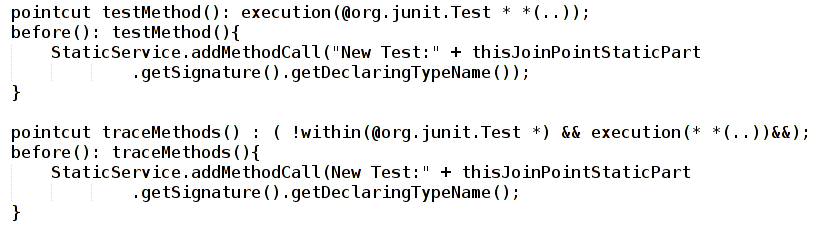
\includegraphics[width = \textwidth]{aspect.png}
\end{center}
\caption{A simplified point cut within AspectJ. The first pointcut is for when a new test is executed and the second when a new method is executed.}
\label{fig:aspectused}
\end{figure}

\section{Framework}
\label{S:framework}

The spectrum of every test has to be compared to that of every other test in order to identify redundant test cases. The metrics identified become computationally heavy with thousands of test cases containing a spectrum consisting of tens of thousands of methods calls. To perform an analysis on that scale would take several days. A pipeline combined with time reduction strategies was determined to be the best solution.

A pipeline approach is shown in Figure \ref{fig:pipeline}. The analysing stages can be set by the user within a properties file, where they can select the spectra type, analysis metric to use and level of redundancy for each. This allows execution of reduction strategies before executing more computationally heavy analysis.

\begin{figure}[h]
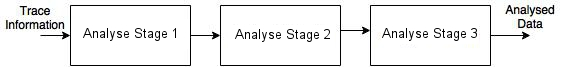
\includegraphics[width=\textwidth]{Pipeline.jpg}
\caption{Trace information goes in at the start of the pipeline. After each stage there will be a reduction of comparisons that the next stage has to complete. The last stages should be the most computationally heavy.}
\label{fig:pipeline}
\end{figure}

There were two approaches that were used to reduce the amount of analysis time. They were - implementing a heuristic and using concurrent execution. 

The heuristic looked at set of method calls, rather than a list. This meant the number of comparisons decreased. Using a 99 percent similarity for the heuristic on the wyc package of Whiley, this decreased the comparisons from stage 1 having \todo{fix these numbers} to stage 2 with . 

The following illustrates an example of this.

$K,I,T,C,H,E,N \neq K,I,T,E,N,Z $

In this case, the two test cases would not be redundant due to them having a large difference in method calls.

$K,I,T,C,H,E,N \approx K,I,T,C,H,N$

There is a chance that these two may be redundant so it implies more computational heavy analysis should be done, such as analysing the list spectra. 

Concurrent execution was implemented by splitting the test cases up into 8 different parts, each part knew the test cases that it had to compare. A new thread was run to execute the comparisons, making the implementation relatively easy. The concurrent execution lead to a decrease in roughly 2 times the time taken to analyse the spectra's but lead to a trade off in an increased memory usage. This meant concurrent execution was only usable for the smaller bench marks.
Another issue was that for each analysis of a benchmark, the tests had to be rerun, this could take several hours. The solution was to save the spectra data to disk. This ensured that a distributed grid system, explored later, can be used to analyse the data.

\section{Benchmarks}
\label{S:bench}
Suitable benchmarks had to be found to test the different metrics on. They were located by looking at popular java framework's, Github repositories and David Pearce's personal projects. The benchmarks had to meet a criteria where they were Java based, had reasonable number of tests (40+) and were open source. Although there were over ten potential benchmarks, the ability to use them depended on their build process. If they used Maven, it was difficult to create a jar that contained the tests and often meant that the amount of effort needed to get a working benchmark was higher than the benefit from it. This eliminated several potential benchmarks and left the Ant and gradle built projects. In Table \ref{large_test} are the large bench marks used. These involved bench marks that required more than \todo{TODO} number of comparisons. The type of tests were also taken into consideration. In Table \ref{small_test} are the smaller bench marks used. A range of sizes were used in order to fully evaluate the framework. Although the framework is more aimed toward larger test suites, it would be interesting to see how it handles smaller test cases and the accuracy it can give. A range of test types was also chosen, David J Pearce's projects contain end to end tests which run through a whole module at once, while the others attempt to test units of code at a time.

\begin{table}[]
\centering
\caption{Large Test Suites}
\label{large_test}
\begin{tabular}{|l|l|l|l|}
\hline
{\bf Benchmark}       &  {\bf Number of Tests} & {\bf Type of tests} & {\bf Authors}   \\ \hline
Whiley - Wyc Valid         &       &    End to End      & David J Pearce          \\ \hline
Spring - Core   &       &    Unit Tests      & Community \\ \hline
Metric-x - Core &       &    Unit Tests      & Community \\ \hline
Jasm              &             &    End to End      & David J Pearce \\ \hline

\end{tabular}
\end{table}

\begin{table}[]
\centering
\caption{Small Test Suites}
\label{small_test}
\begin{tabular}{|l|l|l|l|}
\hline
{\bf Benchmark}   & {\bf Number of Tests} & {\bf Type of tests} & {\bf Authors}  \\ \hline
Ant             &       &    Unit Tests      & Community \\ \hline
Imcache &           &    End to End        & Community \\ \hline
\end{tabular}
\end{table}

\section{Environmental Setup}

As previously discussed in Section \ref{performanceEvalBG} there are a variety of challenges that present themselves when using Java to evaluate the performance of a particular application. \todo{Talk about grid system here. A distributed grid system is used to perform the analysis, this system utilises the computer around the universities that are not currently being used by users. As such, if a user was to log on while a run was being conducted, the application would be paused until the user left. }

\subsection{Measuring Time}
\todo{How to measure time}
Java allows access to a system method that returns the total time in milliseconds from 1970 00:00:00 UTC to the current time. Calling this method before and after the analysing stage allows for the total time taken to analyse to be determined. However, the method has to execute, potentially causing the returned value to slightly off what it actually took. This is also true for the initial time, this time has to be returned and set assigned to a variable, causing a delay between when the analyse starts and the time stored. The time has minimal impact in the context of this framework and will be ignored. Using a distributed grid system has two effects. Firstly, using the system method would not be applicable as this would take into consideration when the application was not running. This was resolved by using the CPU time that the thread had used. Secondly, if a user logs in during analysis, the ram being used by the JVM could potentially be moved into virtual memory dependent on the amount of ram that the user needed. This was limited by running the tests at times when users were unlikely log in such as overnight.

When measuring the time taken to analyse, the start up cost was not taken into account. Running up to 150 jobs concurrently meant that a large number of applications would be attempting to access a single datafile at a single time. This involves a large level of non-deterministic behaviour, to avoid this, the start up cost was not considered.

\subsection{Hardware Environment}
\todo{How to ensure enough heap size}
\todo{How to ensure the same platform used}
\subsubsection{Heap Size}

The heap is the location that the JVM uses to store objects that are produced during the execution of an application. The heap is closely related to the GC. When the size of the heap increases, the number of objects that the garbage collector traverses increases in order to determine which objects should be collected. The amount of heap that was allocated to the JVM was 6gb for every benchmark over every run and was set through the grid system by requiring at least 6gb of free ram before running the process on that machine.

\subsubsection{Platform}

By using a distributed grid system, the platform required had to be specified. The platform that was used was a Linux 4.0.5 64 bit system with 8gb of ram. This was specified through the grid system such that every machine that was used to analyse the data met these requirements.

\subsection{Software Environment}
\todo{Was start up performance calculated into total time?}
\todo{Number of VM invocations?}

A default garbage collection strategy was used. This is known as a concurrent-mark-sweep strategy which uses multiple threads to scan the heap, mark unused objects and recycle them. The approach allows for a high throughput but tends to use more CPU time than other strategies. This was deemed worth the trade off as memory was the bottleneck rather than CPU for the framework and increasing the throughput was more important. \todo{Ref https://docs.oracle.com/javase/8/docs/technotes/guides/vm/gctuning/cms.html}

\section{Method}

This section will go through the process of how the data was retrieved, analysed and evaluated.

Firstly, the benchmarks had to be set up in order to be run the tests locally. This involved retrieving the dependencies of each benchmark and setting up an build script through ant for each, in order to run the tests. After the tests had finished, the trace information was then saved to disk.

The data was then run on a grid computing setup. This setup involves a large number of computers which execute the instructions given to them. Through this, a total of 150 analysing jobs were able to be run concurrently.

Lastly, after the results had been returned, a Wilcoxon signed rank test was used to determine whether the results are significantly different or not. A Wilcoxon signed rank test is a paired difference test that compares two related samples. The significant level used is 95\%. In this paper, the different combinations of techniques to identify redundancy will be as follows:

\begin{itemize}
\item Pipeline size 2 vs Pipeline size 3
\item Parameters vs No Parameters
\item Weighting vs No Weighting
\item Weighting \& Parameters vs Neither
\end{itemize}

A total of seven different property settings were run per benchmark, for example using weighting. Each property setting was run 30 times.